\cotefile{32}
\scanpage{7}
% archive sheet number: 6

4. \uline{Homomorphisme de Gysin}.

Considérons un diagramme commutatif
\noindent(4.1)
\diagram{\begin{tikzcd}[ampersand replacement=\&,column sep=1.1em,row sep=1.5em]
X \handwritten{\arrow[rr,"f"]} \handwritten{\arrow[dr,"p"']} \& \& Y \handwritten{\arrow[dl,"q"]} \\
\& S \&
\end{tikzcd}},
avec $p$ et $q$ compactifiables, \inserted{$p$ plat de prés. finie, \deleted{\unsure{de dim}} $q$ lisse,} $\unsure{S|A}$ étant muni d'un Anneau de torsion $A$ premier aux car. résiduelles. Pour un complexe de $A$-modules $F$ sur $S$, on définit alors un homomorphisme canonique
\[
\handwritten{\mathrm{Tr}_f\ \text{ou}\ }f_{\handwritten{*}}:\quad \mathrm{R}f_{\handwritten{!}}(F_X)\handwritten{\longrightarrow} F_Y(d'-d)\handwritten{[}2(d'-d)\handwritten{]},
\tag*{(4.2)}
\]
en supposant $p,q$ de dimensions relatives $d,d'$ en tout point (il suffit que $p$ soit de dim rel $\handwritten{\leq} d$ en tout point). Si $p$ est également lisse et de dim. rel. exactement $d$ partout, alors \unsure{l'hhomomorphisme|lhhomomorphisme} précédent s'identifie à l'homomorphisme d'adjonction pour $\mathrm{R}f_{\handwritten{!}}$, $\mathrm{R}f^{\handwritten{!}}$ relatif au deuxième membre. En tous cas, l'homomorphisme en question s'appelle \uline{homomorphisme de Gysin} (relatif à $f,F$), ou \uline{homomorphisme trace} (\unsure{parfois} noté $\mathrm{Tr}_f$). On \unsure{appelle|dppelle} encore par le même nom, et on note de même, tout homomorphisme déduit de (4.2) par application d'un foncteur quelconque (le \deleted{cas échéant}\inserted{\handwritten{plus souvent,}} en transformant encore la flèche obtenue en appliquant des isomorphismes canoniques, tels des isomorphismes de transitivité ... , utilisés communément \deleted{\unsure{à|àxà}} comme morphismes d'identification ...). Par exemple on a les homomorphismes
\[
\mathrm{H}^i(f_*)\ \text{ou}\ f_*:\quad \mathbb{R}^i f_{\handwritten{!}}(F_X)\handwritten{\longrightarrow} \underline{\unsure{\mathbb{H}|\mathrm{H}}}^{i\inserted{\handwritten{+2(d'-d)}}}_{\deleted{\unsure{Y|*}}}(F_{\inserted{\handwritten{Y}}})_{\deleted{\unsure{Y|*}}}(d'-d)\deleted{\unsure{[2(d'-d)]}},
\tag*{(4.2.1)}
\]
de faisceaux sur $Y$, déduits de (\unsure{4.2?1|4.2.1}) en appliquant $\underline{\mathrm{H}}^i$, ou
\[
\mathrm{R}q_{\handwritten{!}}(f_{\handwritten{*}})\ \text{ou}\ f_{\handwritten{*}}:\quad \mathrm{R}p_{\handwritten{!}}(F_X)\handwritten{\longrightarrow}\mathrm{R}q_{\handwritten{!}}(F_Y)(d'-d)\handwritten{[}2(d'-d)\handwritten{]},
\tag*{(4.2.2)}
\]
déduit de (4.2) en appliquant $\mathrm{R}q_{\handwritten{!}}$, ou plus généralement, pour tout morphisme \unsure{com\^{p}actifiable|compactifiable}
\[
g:\ Y\handwritten{\longrightarrow}Z
\]
\scanpage{8}
% archive sheet number: 7
\[
\mathrm{R}\handwritten{(}gf_{\deleted{\unsure{!|*}}}\handwritten{)}_{\handwritten{!}}(F_X)\handwritten{\longrightarrow}\mathrm{R}g_{\handwritten{!}}(F_Y)(d'-d)\handwritten{[}2(d'-d)\handwritten{]}\deleted{\unsure{,|.}},
\tag*{(4.2.3)}
\]
déduit de (4.2) en appliquant $\mathrm{R}g_{\handwritten{!}}$. De même, appliquant $\mathrm{R}g_*$, on trouve
\[
\mathrm{R}g_*\mathrm{R}f_{\handwritten{!}}(F_X)\overset{\mathrm{dfn}}{=}\mathrm{R}(gf)_{\deleted{\unsure{!}}c(f)}(F_X)\handwritten{\longrightarrow}\mathrm{R}g_{\handwritten{*}}(F_Y)(d'-d)\handwritten{[}2(d'-d)\handwritten{\unsure{]} }
\tag*{(4.2.4)}
\]
(où la \deleted{premier}\inserted{source} est ``l'image directe à supports propres sur $Y^{\deleted{\unsure{*}}}$'' )\deleted{\unsure{, qui}}

\deleted{Prenant en particulier} Pour définir cette dernière flèche, \deleted{il était}\inserted{quitte à faire rentrer le $(d'-d)$ dans la parenthèse, il} suffisait de disposer d'un morphisme de \deleted{sites} topos $Y_{\text{ét}}\handwritten{\longrightarrow}Z$, et prenant alors pour $Z$ le topos final, on trouve l'exemple important d'homomorphisme de Gysin:
\[
\mathrm{R}\handwritten{\Gamma}_X(\mathrm{R}f_{\handwritten{!}}(F_X))\overset{\mathrm{dfn}}{=}\mathrm{R}\handwritten{\Gamma}_{X,\deleted{\unsure{!}}c(f)}(F_X)\handwritten{\longrightarrow}\mathrm{R}\handwritten{\Gamma}_Y(F_Y(d'-d))\handwritten{[}2(d'\unsure{-|\mathord{\perp}}d)\handwritten{\unsure{]} }
\tag*{(4.2.5)}
\]
Dans le cas où $f$ est \uline{propre}, (4.2) devient
\[
\mathrm{R}f_{\handwritten{*}}(F_X)\handwritten{\longrightarrow}\mathbb{F}_Y(d'-d)\handwritten{[}2(d'-d)\handwritten{]},
\tag*{(4.2.\unsure{6|5})}
\]
et (4.2.4) et (4.2.5) s'écrivent respectivement
\[
\mathrm{R}(gf)_*(F_X)\handwritten{\longrightarrow}\mathrm{R}g_{\handwritten{*}}(F_Y)(d'-d)\handwritten{[}2(d'-d)\handwritten{]},
\tag*{(4.2.7)}
\]
\[
\mathrm{R}\handwritten{\Gamma}_X(F_X)\handwritten{\unsure{\text{---}|\longrightarrow}}\mathrm{R}\Gamma_Y(F_Y(d'-d))\handwritten{[}2(d'-d)\handwritten{]}.
\tag*{(4.2.8)}
\]

\deleted{Dans (4.2.5) ou (4.2.8), il y aurait lieu de remplacer $F_X$ par un $F_X(i)$} On a également à définir des homomorphismes de Gysin pour des coéfficients sur $Y$ plus généraux que ceux de la forme $F_Y$ et ceux qu'on en déduit par twist et shift. De façon générale, soit $G$\unsure{.} un complexe de $A$-Modules (NB je ne précise pas ici\inserted{ni ailleurs} les hypothèses de degré) sur $Y$, et appliquons à (4.2) le foncteur $\overset{\mathrm{L}}{\otimes}G$, on trouve un homomorphisme canonique, qui est d'ailleurs le même que si on partait de \deleted{\unsure{F}} $F'=A_S$ sur $S$, et qu'on tensorise l'homomorphisme de Gysin correspondant par $F_Y\otimes G$. Donc, autant oublier $F$ et dire que pour tout $G$ sur $Y$, on a un homomorphisme canonique (dit\inserted{\handwritten{encore}} \uline{de Gysin})
\margin{\handwritten{\fbox{\parbox{1.8cm}{Question: a-t-on besoin d'un $A$ sur $S$, \unsure{ou|ne} suffit d'avoir un Anneau $A_Y$ sur $Y$, de torsion, premier à $Y$ ?}}}}
\[
\boxed{\mathrm{R}f_{\handwritten{!}}(f^{\handwritten{*}}(G))\handwritten{\longrightarrow}G(d'-d)\handwritten{[}2(d'-d)\handwritten{]}},
\tag*{(4.3)}
\]
ou, au choix
\scanpage{9}
% archive sheet number: 8
\[
\mathrm{R}f_{\handwritten{!}}(\handwritten{f^*}G(d-d'))\handwritten{\longrightarrow}G\handwritten{[}2(d'-d)\handwritten{]}.
\tag*{(4.3 bis)}
\]
Arrivé à ce point, je constate que c'est par cette flèche\inserted{(4.3)} (plus raisonnable que (4.2)) qu'il aurait fallu commencer, en ajoutant encore que si $p$ est également lisse et est de \unsure{dim,|dim;} rel. $d$ partout, \deleted{alors (\unsure{4.3|4.2})}\inserted{et si $G$ est localement (sur $Y_{\text{ét}}$) isomorphe à l'image inverse d'un complexe sur $S$, alors (4.3)} s'identifie à l'homomorphisme d'adjonction qu'on pense. Il y aurait lieu alors de donner les exemples (4.2.1) à (4.2.8) \deleted{\unsure{du|de}} en partant de (4.3) plutôt que de (4.2). On peut laisser tomber (4.2.1), et se borner à dire que les homomorphismes déduits des homomorphismes envisagés par application des foncteurs $\mathrm{H}^i$ sont également affublés du nom ``Gysin'' ou ``trace''.

\unsure{Une|Upe} perplexité: dans le contexte actuel, la notation $f_{\handwritten{*}}$, qui dénote à la fois un foncteur (image directe) et un homomorphisme de foncteurs (Gysin) ne semble pas bien fameux. Je propose de donner la préférence ici à la notation $\mathrm{Tr}_f$, en le disant au moment ou on signale également la notation $f_{\handwritten{*}}$.

Etant donné le nombre d'exemples parmi les variantes à Gysin, il est clair qu'il ne sera pas possible de donner un formulaire qui donne\inserted{rait} \deleted{immédiatement} sans déductions du tout, tous les cas qu'on rencontrera. Il faudra se borner à donner un formulaire directement en termes des homomorphismes de Gysin fondamentaux sous la forme (4.3), et se borner à donner comme exemple la forme \unsure{qae|que} prend ce formulaire\handwritten{``}après application d'un foncteur $\mathrm{R}g_*$\handwritten{''} dans le cas $f$ propre, disons.

Voici des points qui doivent certainement figurer au formulaire:

\margin{\handwritten{descend}}
\deleted{\unsure{a}}\handwritten{d}) Compatibilité avec la formule de projection: Si on a un complexe de modules $G'$ sur $Y$ et si on tensorise (4.3) par $G'$, en utilisant la formule de projection de XVII ... , on trouve Gysin pour $G\overset{\mathrm{L}}{\otimes}G'$. Ceci \deleted{montre}\inserted{\handwritten{\unsure{contient}}} en particulier que, via la formule de projection,
\scanpage{10}
% archive sheet number: 9
(4.3) est connu pour tout $G$ par la seule connaissance de
\[
\mathrm{R}f_{\handwritten{!}}(A_X(d-d')\handwritten{[}2(d-d')\handwritten{]})\handwritten{\longrightarrow}A_Y.
\tag*{(4.4)}
\]
Ceci devrait bien donner la formule de projection au niveau des classes de cohomologie (qu'il faut bien entendu expliciter, soit ici, soit\inserted{(mieux)} à la fin du formulaire, en reprenant ce formulaire dans \deleted{\unsure{le ca}} le cas particulier recommandé\handwritten{,} parmi les variantes possibles).

\deleted{\unsure{b}}\handwritten{a}) \uline{Si} $d=d'$ \uline{et si} $\unsure{g|f}$ \uline{est quasi-fini} (et alors automatiquement plat, supposant que la dimension relative de $p$ est partout $d$), alors on retrouve l'homomorphisme trace de XVII ...

\deleted{\unsure{c}}\handwritten{b}) Si $f$ \uline{est lisse}, on retrouve l'homomorphisme trace du par.2.

\deleted{\unsure{d}}\handwritten{c}) \uline{Transitivité} pour un composé $gf$ ($g:Y\handwritten{\longrightarrow}Z$, avec $Z$ lisse et compactifiable sur $S$).

\margin{\handwritten{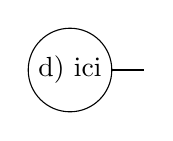
\begin{tikzpicture}\node[draw,circle,inner sep=2pt] (n) {d) ici};\draw (n.east)--++(0.4,0);\end{tikzpicture}}}
\deleted{\unsure{e}}\handwritten{f}) Compatibilité avec \uline{Künneth}, quand on regarde $g_1\mathbin{\mathrm{x}}_S g_2:X_1\mathbin{\mathrm{x}}_S X_2\handwritten{\longrightarrow}Y_1\mathbin{\mathrm{x}}_S Y_2$. Compatibilité avec \uline{changement de base}\inserted{$S'\handwritten{\longrightarrow}S$.}

\deleted{\unsure{f}}\handwritten{e}) Compatibilité avec \uline{changement d'Anneau} $A\handwritten{\longrightarrow}A'$ (qui \unsure{montre} qu'il suffit de connaitre (4.4) pour les $A=(\underline{\mathrm{Z}}/n\underline{\mathrm{Z}})_S$ pour l'avoir pour tout $A$).

 g) \uline{Indépendance par rapport à} $S$ (si on se donne $S\handwritten{\longrightarrow}\deleted{\unsure{S|et}}T$ lisse, de sorte que l'on peut regarder $X$ et $Y$ comme étant sur $T$ ...).

 h) \uline{Formule d'échange}, relatif au cas où on a un diagramme cartésien
\diagram{\begin{tikzcd}[ampersand replacement=\&,row sep=2em,column sep=2em,execute at end picture={\draw[gray] ([xshift=-2pt,yshift=6pt]xx.north west) .. controls ([xshift=-22pt,yshift=10pt]xx.west) and ([xshift=-18pt,yshift=-14pt]yy.west) .. ([yshift=-12pt]yy.south) .. controls ([xshift=25pt,yshift=-16pt]yyp.south) and ([xshift=20pt,yshift=12pt]yyp.east) .. ([yshift=12pt]yyp.north) .. controls ([xshift=-10pt,yshift=20pt]yyp.north) and ([yshift=-14pt]xx.east) .. ([xshift=9pt]xx.north east);}]
|[alias=xx]| X \handwritten{\arrow[d,"f"']} \& X' \handwritten{\arrow[l,"h"']} \handwritten{\arrow[d,"f'"]} \\
|[alias=yy]| Y \& |[alias=yyp]| Y' \handwritten{\arrow[l,"g"']}
\end{tikzcd}}
de schémas sur $S$: appliquant $g^*$ à $\mathrm{Tr}_f$, et appliquant \deleted{\unsure{la for}} l'isomorphisme de changement de base pour $\mathrm{R}f_{\handwritten{!}}$ et $g^*$, on doit trouver $\mathrm{Tr}_{f'}$. On supposera bien sûr $Y$ et $Y'$ lisses sur $S$, $X$ plat sur $S$, et pour que $X'$ soit plat sur $S$, il faut évidemment une hypothèse genre Tor-indépendance de $X$ et $Y'$ sur $Y$. Cela doit marcher en tous cas si $X$ est également lisse sur $S$, et si $f$ et $g$ sont \uline{transversaux} (EGA IV \unsure{17|27}...).
\scanpage{12}
% archive sheet number: 11
 i) \uline{Formule d\deleted{'}e}\deleted{adjonction}\inserted{\uline{transposition ou d'adjonction}}, disant que Gysin \deleted{est} sur la cohomologie à supports propres est transposé de l'homomorphisme image inverse. J'ai un sentiment que cela résulte tautologiquement de la définition, \deleted{\unsure{et n'a} guère de sens que dans}

 j) \uline{Formules de \unsure{finéarité|linéarité}} (notamment pour $f$ une immersion de schémas relatifs lisses)\handwritten{,} nécessaire pour Jouanolou; regarder aussi la formule de linéarité pour variété\deleted{s} éclatée\deleted{s} déduite\deleted{s} de cette situation. Si possible, donner formulation commune ?

Comme plan possible du par.4, je vois

4.1. Définition et notations.

4.2. Formulaire général.

4.3. Formulaire spécial\deleted{\unsure{s|e}}, pour classes de cohomologie.

Du point de vue notations, je suggère, pour ne pas trainer indéfiniment des $d-d'$ dans les notations, de travailler systématiquement avec la \uline{dimension virtuelle} $d(f)=d-d'$ de $f$; c'est elle qui mérite une lettre simple, telle que $d$.

Dans 4.3, inclure le cas $f$ propre, $d=d'$; dire que dans ce \deleted{5. \uline{Classes fondamentales locales}} cas on a
\[
\mathrm{Tr}_f(1_X)=N\,1_Y
\]
\margin{\handwritten{\begin{tikzpicture}\draw[gray] (0,0) .. controls (-0.7,1) and (-0.7,2.5) .. (0,3.4);\end{tikzpicture}}}
où $N$ est une fonction entière localement constante sur $Y$, appelée \uline{degré} de $f$, et qu'on peut caractériser comme étant égale, sur \deleted{tout} le plus grand ouvert de $Y$ sur lequel $f$ soit fini localement libre, comme égale au degré habituel. Conclure que $\mathrm{Ker}(f^{\handwritten{*}}:\mathrm{H}^{\handwritten{\unsure{*|+}}}(Y,G)\handwritten{\longrightarrow}\mathrm{H}^{\handwritten{*}}(X,G_X))$ est annulé par $N$, donc\inserted{\handwritten{$f^*$}} est injectif (et même inversible à gauche) si $N=1$. \handwritten{[}Si $S=\mathrm{Spec}\,k$ et si $Y$ est irréductible, de point générique $\handwritten{\eta}$,\inserted{\handwritten{($d$ et $d'$ quelconques)}} et si $N$ est le pgcd des degrés des $0$-cycles de $X_{\handwritten{\eta}}$\inserted{\handwritten{$\neq\varnothing$}}, on peut de même trouver un homomorphisme\handwritten{,} fonctoriel en $G$\handwritten{\unsure{$\leftarrow$}}\handwritten{,} $\mathrm{H}^{\handwritten{*}}(X,G_X)\handwritten{\longrightarrow}\mathrm{H}^{\handwritten{*}}(Y,G)$ dont le composé avec l'homomorphisme image inverse est $N.\mathrm{id}$.\handwritten{]}
\scanpage{13}
% archive sheet number: 12
5. \uline{Classe fondamentale locale}.

Reprenons l'homomorphisme de Gysin général (4.3), et \unsure{notans|notons} que par la formule d'adjonction, sa connaissance équivaut à celle d'un homomorphisme
\[
f^{\handwritten{*}}(G)(d-d')\handwritten{[}2(d-d')\handwritten{]}\handwritten{\unsure{\Longrightarrow|\longrightarrow}}\mathrm{R}f^{\handwritten{!}}G,
\tag*{(4.4)}
\]
\margin{\handwritten{\tikz[baseline=(n.base)]{\node[rotate=12] (n) {autre nom?};\draw[rotate=12] (0,0) ellipse (1.15cm and .35cm);}}}
\deleted{\unsure{qui, pour $f$}}\handwritten{[}On l'appelle l'homomorphisme \uline{classe fondamentale locale}(?)\handwritten{]}. Il est fonctoriel en $G$, et, comme nous avons vu au par.4, il suffit de le connaitre pour $G=A_Y$ pour le connaitre pour tout $G$. Dans ce cas, on peut l'interpréter comme un homomorphisme
\[
\handwritten{\phi}_f:\quad A_X\handwritten{\longrightarrow}\mathrm{R}f^{\handwritten{!}}(A_Y)(d'-d)\ 2(d'-d)\handwritten{,}\quad\deleted{\text{\unsure{sur}}\ \unsure{\phi_Y|Y}}
\tag*{(4.5)}
\]
\inserted{\handwritten{i.e. }$\handwritten{\varphi_f\in}\mathrm{H}^{\handwritten{2}(d-d')}(Y,\mathrm{R}f^{\handwritten{!}}(A_Y)(d-d'))$}
et il définit par suite une section, notée de même
\[
\begin{aligned}
&\deleted{\underline{\handwritten{\phi}}_f\ \handwritten{\unsure{\leftarrow|\in}}\ \mathrm{H}^0(Y,\underline{\mathrm{H}}^0(\mathrm{R}f^{\handwritten{!}}(A_Y)(d'-d)\ 2(d'-d))}\quad\\
&\inserted{\handwritten{\varphi_f\in}\mathrm{H}^0(Y,\underline{\mathbb{R}}^{\handwritten{2}(d'-d)}(\deleted{\mathrm{R}}f^{\handwritten{!}}(A_Y))(d'-d))},
\end{aligned}
\tag*{\tikz[baseline=(n.base)]{\node (n) {(4.6)};\handwritten{\draw[gray] (-.65,-.85) .. controls (-.42,-.9) and (-.8,.15) .. (-.6,.3) .. controls (-.25,.65) and (.45,.6) .. (.65,.3) .. controls (.72,.12) and (.55,-.55) .. (.55,-.77) -- (.73,-.81);}}}
\]
qu'on appelera également (et peut-être à meilleur escient) la \uline{classe fondamentale locale} \uline{pour} $f$. On notera que pour la connaitre pour tout $A$, il suffit de la connaitre pour les $\underline{\mathrm{Z}}/n\underline{\mathrm{Z}}$ (du moins si on se borne aux $A$ qui sont annulés par un même entier $n\handwritten{\geq}1$ premier aux car. résiduelles de $S$): \deleted{La connaissance de (4.6) permet de reconstituer} plus précisément, la formation des classes $\handwritten{\phi}_f$ de (4.5) et de (4.6) est \uline{fonctoriel} en l'Anneau $A_S$ (voire, en $A_Y$).

Lorsqu'on dispose d'une ``formule de pureté''
\[
\deleted{\unsure{\underline{\mathrm{H}}^i(\mathrm{R}|\underline{\mathrm{H}}^i\mathrm{R}}}\ \mathrm{R}^i f^{\handwritten{!}}(A_Y)=0\quad\text{pour }i\handwritten{<}2(d-d'),
\tag*{(4.7)}
\]
la connaissance de (4.6) équivaut même à celle de (4.5), ce dernier $\handwritten{\phi}_f$ méritant le nom de \uline{classe fondamentale globale} de $X$ sur $Y$.

Nous allons nous intéresser par la suite au cas où $f:X\handwritten{\longrightarrow}Y$ est une \uline{immersion fermée}. On sait alors que les formules de pureté (4.7)
\scanpage{14}
% archive sheet number: 13
sont vérifiées. (Lorsque $X$ est également lisse, c'est contenu dans XVI 3.7 ; le cas général - sans même supposer $Y$ plat sur $S$, d'ailleurs - s'en déduit par \deleted{\unsure{un|du}} dévissage facile, et il est traité d'ailleurs dans SGA 2 XIV 1, conjonction de 1.10 et de 1.18.) La classe $\handwritten{\phi}_f$ de (4.5) peut alors s'interpréter aussi comme un élément \deleted{\unsure{de|du}}
\[
\deleted{\handwritten{\phi}_f}\handwritten{\gamma_{X/Y}\in}\mathrm{H}^{\handwritten{2}(d-d')}_{\inserted{\handwritten{X}}}(\handwritten{\unsure{Y|X}},A_{\handwritten{Y}}(d-d')).
\tag*{(4.8)}
\]
Cette classe s'appelle la \uline{classe de cohomologie à supports dans} $X$ \uline{de} $X$ \uline{dans} $Y$, et son image
\[
\handwritten{\gamma}_{X/Y}\handwritten{\in}\mathrm{H}^{\handwritten{2}(d-d')}(Y,A_Y(d-d'))
\tag*{(4.9)}
\]
\uline{la classe de cohomologie} (sous-entendue: à supports quelconques) \uline{de} $X$ \uline{dans} $Y$. Le formalisme des classes de cohomologie\inserted{\handwritten{(4.8) (4.9)}} ainsi \deleted{associées}\inserted{\handwritten{obtenues}} \deleted{aux} (une fois la définition étendue par linéarité à des cycles algébriques relatifs sur $Y$) sera étudié systématiquement dans SGA 5 IV. Notre propos ici est d\unsure{è|é|e}\deleted{n} donner \deleted{certaines pr} les propriétés les plus élémentaires de la classe locale (4.6), en attachant notre attention surtout au cas où $X$ est également lisse sur $S$.

Voici une liste de propriétés à expliciter qui me semble raisonnable\deleted{\unsure{;|:}} (où on pose $\deleted{p}\handwritten{\delta}=d-d'$)\deleted{;}:

 a) Si $X$ est lisse sur $S$, et si $G$ est localement\inserted{(ét)} sur $Y$ isomorphe à l'image inverse d'un complexe sur $S$,\inserted{\handwritten{p.ex. $G=(A)_Y$,}} alors (4.4) est un isomorphisme. (C'est essentiellement contenu dans XVI 3.7).

 b) Si $\deleted{p}\handwritten{\delta}=0$ i.e. $f$ un isomorphisme, (4.4) est l'identité i.e. $\handwritten{\phi}_f=1$ dans (4.5) ou (4.6).

\tikz[baseline=(c.base)]{\node (c) {c)};\handwritten{\draw (c.center) ellipse (.4cm and .5cm);}} Si $\deleted{p}\handwritten{\delta}=1$, de sorte que $X$ est un diviseur relatif sur $Y/S$, alors $\handwritten{\phi}_f$ de (4.5) i.e. (4.8), et a fortiori de (4.6) ou (4.9), est donné par la théorie de Kummer comme d'habitude.

 d) Compatibi\unsure{m|l}ité de $\handwritten{\phi}_f$ avec \uline{transitivité} et \uline{intersections} (\unsure{ces|ves} deux formules sont essentiellement identiques), dans le cas \uline{lisse}\handwritten{\unsure{,|;}}
\scanpage{15}
% archive sheet number: 14
\margin{\handwritten{\figure{\begin{tikzpicture}\draw[gray] (0,.55) .. controls (.02,.35) and (.12,.15) .. (.2,.1);\draw[gray,densely dashed] (.43,.17) .. controls (.5,.38) and (.54,.62) .. (.58,.8);\end{tikzpicture}}}}
\uline{et transversal}.

 e) $\unsure{\mathbb{C}|\mathrm{C}}$ompatibilité avec \uline{changement de base} $S'\handwritten{\longrightarrow}S$, avec \uline{produits cartésiens} $Y_1\mathbin{\mathrm{x}}_S Y_2$ sur $S$.

\unsure{g|f}) Indépendance par rapport à $S$. \handwritten{($S\unsure{\text{---}|\longrightarrow}T$)}
\margin{\handwritten{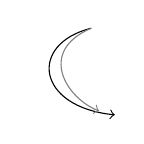
\begin{tikzpicture}\draw[->] (0,1.1) .. controls (-.8,.9) and (-.7,.1) .. (.3,0);\draw[gray,->] (0,1.1) .. controls (-.7,.8) and (-.3,.2) .. (.1,.05);\end{tikzpicture}}}

 f) Compatibilité avec changement d'anneau.

 h) \unsure{Remation|Relation} avec Gysin: Les classes (4.8),(4.9) s'interprètent comme l'image de $1_X$ par Gysin. Le transformé de (4.4) par $\mathrm{R}f_{\handwritten{!}}$, suivi de l'homomorphisme d'adjonction, est l'homomorphisme de Gysin.

Je pense que, compte tenu du formulaire de par.4, le formulaire \deleted{ici} proposé ici pour les classes fondamentales $\pm$ locales est pratiquement trivial\deleted{\unsure{,|e}} à partir des définitions. On peut \deleted{\unsure{don|donc}}, pour finir, récupérer un énoncé qui donne la \uline{caractérisation} des classes fondamentales locales dans le cas d'un couple lisse, par les propriétés suivantes 1) Nature locale (pour Zar suffit) 2) cas $p=0$ 3) cas $p=1$, quand $X$ est défini par une équation 4) propriété de cup-produit d) (où il suffit de \unsure{preddre|prendre} un des deux facteurs de codimension 1). Signaler\inserted{en remarque} que cet énoncé\deleted{\unsure{,}}\inserted{(existence et unicité d'une théorie des cl. fond. loc.)} peut se démontrer sans difficulté indépendamment de la théorie de dualité et de celle de l'homomorphisme trace, et avait été donnée dans le séminaire oral \deleted{\unsure{au prélimi|au prélim}} avant la dualité.

Remords: il serait pr\unsure{\.{u}|u}dent d'adjoindre au formulaire un
\margin{\handwritten{\begin{tikzpicture}\draw[->] (.3,0) .. controls (-1.4,2.4) and (-1.1,4.6) .. (.3,5.2);\draw (.4,.4)--(-.12,.1);\draw (-.12,.1) .. controls (-.8,-.8) and (-.6,-2.8) .. (-.7,-3.6) .. controls (-.7,-3.9) and (-.3,-3.9) .. (-.2,-3.9);\end{tikzpicture}}}

 i) On a commutativité dans le diagramme suivant
\diagram{\begin{tikzcd}[ampersand replacement=\&,column sep=3em,row sep=2em]
f^*(G)(\inserted{\handwritten{-}}p)\handwritten{[}\inserted{\handwritten{-}}2p\handwritten{]} \handwritten{\arrow[r]} \handwritten{\arrow[dr,bend right=18]} \& \mathrm{R}f^{\handwritten{!}}(G) \\
\& \mathrm{R}f^{\handwritten{!}}(A_Y)\overset{\underline{\mathrm{L}}}{\otimes}{\unsure{f|g}}^{\handwritten{*}}(G) \handwritten{\arrow[u]}
\end{tikzcd}},
où la flèche horizontale est (4.4), la flèche oblique est déduite par $\overset{\underline{\mathrm{L}}}{\otimes}G$ de (4.\unsure{5|9}),\deleted{dans le cas} et le flèche verticale est l'homomorphisme canonique qu'on devine,\deleted{et} analogue à celui de changement de base pour les \handwritten{$!$}, et qui manque dans 3.1\handwritten{(}tout comme ce dernier\handwritten{)}. On s'y intéressera sans doute surtout si $G$ est localement libre, donc l'homomorphisme en question est un isomorphisme.
